\documentclass[aspectratio=169]{beamer}
% Theme and color scheme
\usetheme{Antibes}
\usecolortheme{beaver}


% Packages
\usepackage[utf8]{inputenc}
\usepackage[T1]{fontenc}
\usepackage{graphicx}
\usepackage{listings}
\usepackage{xcolor}
\usepackage{colortbl}
\usepackage{tikz}
\usepackage{hyperref}
\usetikzlibrary{shapes,arrows,positioning}

% Java code highlilsts
\lstset{
    language=Java,
    basicstyle=\ttfamily\small,
    keywordstyle=\color{blue}\bfseries,
    commentstyle=\color{green!60!black},
    stringstyle=\color{red},
    numberstyle=\tiny\color{gray},
    numbers=left,
    breaklines=true,
    showstringspaces=false,
    tabsize=2,
    frame=single,
    backgroundcolor=\color{gray!10}
}

% Title information
\title{Java Fundamentals Review}
\subtitle{If Statements, Data Types, and Operations}
\author{Aadrit Talukdar, Nikola Mazzola, Arjun Maganti, Harish Senthilkumar}
\institute{Basis Independent Silicon Valley}
\date{August 20, 2025}

% Remove navigation symbols
\setbeamertemplate{navigation symbols}{}

\begin{document}

% Title slide
\begin{frame}
    \titlepage
\end{frame}

% Table of contents
\begin{frame}{Agenda}
    \tableofcontents
\end{frame}

% Section 1: If Statements
\section{If Statements}

\begin{frame}[fragile]{If Statements}
    \frametitle{If Statements in Java}
    
    \begin{columns}
        \begin{column}{0.7\textwidth}
            \begin{itemize}
                \item If statements allow programs to make decisions
                \item They control the flow of execution based on conditions
                \item Essential for creating dynamic, responsive programs
            \end{itemize}
            
            \vspace{0.5em}
            
            \textbf{Basic Syntax:}
            \begin{lstlisting}
if (condition) {
    // runs if condition is true
}
            \end{lstlisting}
            
            \small \textbf{Note:} Condition must evaluate to a boolean value (true or false).
        \end{column}
        
        \begin{column}{0.3\textwidth}
            \begin{center}
                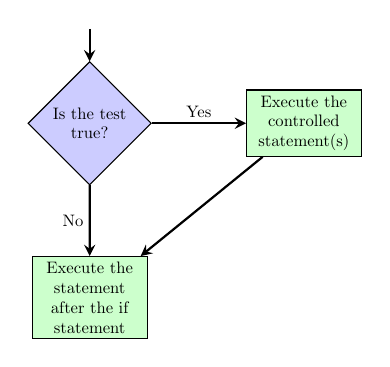
\begin{tikzpicture}[node distance=1.2cm, auto, >=stealth, scale=0.6, transform shape]
                    % Define styles
                    \tikzstyle{decision} = [diamond, draw, fill=blue!20, text width=1.8cm, text badly centered, inner sep=1pt]
                    \tikzstyle{process} = [rectangle, draw, fill=green!20, text width=2.2cm, text centered, minimum height=0.6cm]
                    \tikzstyle{line} = [draw, ->, thick]
                    
                    % Nodes
                    \node [decision] (test) {Is the test true?};
                    \node [process, right=2cm of test] (execute_if) {Execute the controlled statement(s)};
                    \node [process, below=1.5cm of test] (execute_after) {Execute the statement after the if statement};
                    
                    % Arrows
                    \draw [line] (0,2) -- (test);
                    \draw [line] (test) -- node [above] {Yes} (execute_if);
                    \draw [line] (test) -- node [left] {No} (execute_after);
                    \draw [line] (execute_if) -- (execute_after);
                \end{tikzpicture}
            \end{center}
        \end{column}
    \end{columns}
\end{frame}

\begin{frame}[fragile]{If-Else Statements}
    \frametitle{If-Else Statements}
    
    \begin{columns}
        \begin{column}{0.5\textwidth}
            \begin{lstlisting}
if (condition) {
    // code if true
} else {
    // code if false
}
            \end{lstlisting}
            
            \vspace{0.5em}
            If-else provides an alternative path when the condition is false.
        \end{column}
        
        \begin{column}{0.5\textwidth}
            \begin{center}
                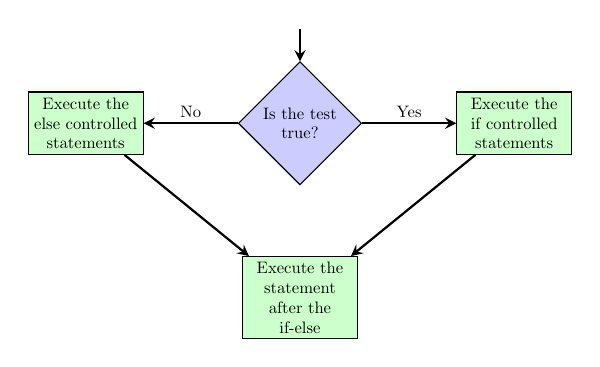
\begin{tikzpicture}[node distance=1.2cm, auto, >=stealth, scale=0.6, transform shape]
                    % Define styles
                    \tikzstyle{decision} = [diamond, draw, fill=blue!20, text width=1.8cm, text badly centered, inner sep=1pt]
                    \tikzstyle{process} = [rectangle, draw, fill=green!20, text width=2.2cm, text centered, minimum height=0.6cm]
                    \tikzstyle{line} = [draw, ->, thick]
                    
                    % Nodes
                    \node [decision] (test) {Is the test true?};
                    \node [process, right=2cm of test] (execute_if) {Execute the if controlled statements};
                    \node [process, left=2cm of test] (execute_else) {Execute the else controlled statements};
                    \node [process, below=1.5cm of test] (execute_after) {Execute the statement after the if-else};
                    
                    % Arrows
                    \draw [line] (0,2) -- (test);
                    \draw [line] (test) -- node [above] {Yes} (execute_if);
                    \draw [line] (test) -- node [above] {No} (execute_else);
                    \draw [line] (execute_if) -- (execute_after);
                    \draw [line] (execute_else) -- (execute_after);
                \end{tikzpicture}
            \end{center}
        \end{column}
    \end{columns}
\end{frame}

\begin{frame}[fragile]{If-Else-If Chains}
    \frametitle{Multiple Conditions with Else-If}
    
    \begin{columns}
        \begin{column}{0.5\textwidth}
            \begin{lstlisting}
if (condition1) {
    // code for condition1
} else if (condition2) {
    // code for condition2
} else {
    // default code
}
            \end{lstlisting}
            
            \vspace{0.5em}
            Else-if chains allow testing multiple conditions in sequence.
        \end{column}
        
        \begin{column}{0.5\textwidth}
            \begin{center}
                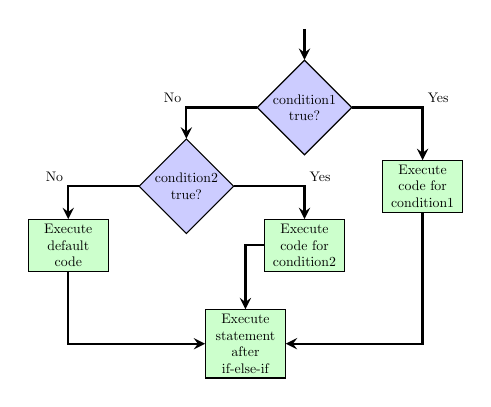
\begin{tikzpicture}[node distance=1cm, auto, >=stealth, scale=0.5, transform shape]
                    % Define styles
                    \tikzstyle{decision} = [diamond, draw, fill=blue!20, text width=1.6cm, text badly centered, inner sep=1pt]
                    \tikzstyle{process} = [rectangle, draw, fill=green!20, text width=1.8cm, text centered, minimum height=0.5cm]
                    \tikzstyle{line} = [draw, ->, thick]
                    
                    % Nodes positioned in cascade from top-right to bottom-left
                    \node [decision] (test1) at (3,3.5) {condition1 true?};
                    \node [process] (execute1) at (6,1.5) {Execute code for condition1};
                    \node [decision] (test2) at (0,1.5) {condition2 true?};
                    \node [process] (execute2) at (3,0) {Execute code for condition2};
                    \node [process] (execute_else) at (-3,0) {Execute default code};
                    \node [process] (execute_after) at (1.5,-2.5) {Execute statement after if-else-if};
                    
                    % Arrows with right angles - no diagonals
                    \draw [line] (3,5.5) -- (test1);
                    % Yes from condition1 - right then down to execute1
                    \draw [line] (test1) -| node [above right] {Yes} (execute1);
                    % No from condition1 - left then down to test2
                    \draw [line] (test1) -| node [above left] {No} (test2);
                    % Yes from condition2 - right then down to execute2
                    \draw [line] (test2) -| node [above right] {Yes} (execute2);
                    % No from condition2 - left then down to else
                    \draw [line] (test2) -| node [above left] {No} (execute_else);
                    
                    % All paths converge to final statement
                    \draw [line] (execute1) |- (execute_after);
                    \draw [line] (execute2) -| (execute_after);
                    \draw [line] (execute_else) |- (execute_after);
                \end{tikzpicture}
            \end{center}
        \end{column}
    \end{columns}
\end{frame}

\begin{frame}{If Statements - Exercise 1}
    \frametitle{Exercise: Grade Calculator}
    
    \textbf{Task:} Write a program that takes a numerical grade and outputs the corresponding letter grade.
    
    \vspace{1em}
    
    \textbf{Grading Scale:}
    \begin{itemize}
        \item 90-100: A
        \item 80-89: B
        \item 70-79: C
        \item 60-69: D
        \item Below 60: F
    \end{itemize}

\end{frame}

\begin{frame}[fragile]{If Statements - Solution 1}
    \frametitle{Solution: Grade Calculator}
    
    \begin{lstlisting}
if (grade <= 100 && grade >= 90) {
    System.out.println("A");
} else if (grade >= 80) {
    System.out.println("B");
} else if (grade >= 70) {
    System.out.println("C");
} else if (grade >= 60) {
    System.out.println("D");
} else if (grade < 60 && grade >= 0) {
    System.out.println("F");
} else {
    System.out.println("Invalid grade");
}

    \end{lstlisting}
    
    % TODO: Add explanation of the solution
\end{frame}

% Section 2: Data Types
\section{Data Types}

\begin{frame}{Data Types Overview}
    \frametitle{Java Data Types}
    
    \begin{block}{Definition: Data Types}
        A name for a category of data values that are all related, as in type int in Java, which is used to represent integer values.
    \end{block}
    
    \vspace{0.5em}
    
    \textbf{Why are Data Types Important?}
    \begin{itemize}
        \item Every variable in Java must have a declared data type
        \item Java is a strongly typed language - data types are enforced at compile time
        \item Help prevent errors by ensuring operations are performed on compatible data
    \end{itemize}
    
    
\end{frame}

\begin{frame}{Primitive Data Types}
    \frametitle{Primitive Data Types in Java}
    
    \textbf{What are Primitive Data Types?}
    \begin{itemize}
        \item Built-in data types provided by Java
        \item Store simple values directly in memory
        \item Eight primitive data types in Java
    \end{itemize}
    
    \vspace{0.5em}
    
    \begin{table}[h]
        \centering
        \small
        \rowcolors{2}{blue!10}{white}
        \begin{tabular}{|l|l|l|}
            \hline
            \rowcolor{blue!30}
            \textbf{\color{white}Type} & \textbf{\color{white}Description} & \textbf{\color{white}Examples} \\
            \hline
            \texttt{\textbf{byte}} & 8-bit integer (-128 to 127) & \texttt{byte age = 25;} \\
            \hline
            \texttt{\textbf{short}} & 16-bit integer (-32,768 to 32,767) & \texttt{short year = 2024;} \\
            \hline
            \texttt{\textbf{int}} & 32-bit integer (most common) & \texttt{int score = 95;} \\
            \hline
            \texttt{\textbf{long}} & 64-bit integer (very large numbers) & \texttt{long population = 8000000000L;} \\
            \hline
            \texttt{\textbf{float}} & 32-bit decimal number & \texttt{float price = 19.99f;} \\
            \hline
            \texttt{\textbf{double}} & 64-bit decimal (more precise) & \texttt{double pi = 3.14159;} \\
            \hline
            \texttt{\textbf{boolean}} & True or false values & \texttt{boolean isActive = true;} \\
            \hline
            \texttt{\textbf{char}} & Single character (16-bit Unicode) & \texttt{char grade = 'A';} \\
            \hline
        \end{tabular}
    \end{table}
\end{frame}

\begin{frame}[fragile]{Numeric Data Types}
    \frametitle{Working with Numbers}
    
    \textbf{Understanding Numeric Types and Their Uses:}
    \begin{itemize}
        \item Choose the right type based on the range of values you need
        \item Consider memory usage for large datasets
        \item Be aware of precision differences between float and double
    \end{itemize}
    
    \begin{lstlisting}
int age = 18;                    // Most common for whole numbers
double price = 29.99;            // Default for decimal numbers
long population = 7800000000L;   // Need 'L' suffix for long literals
float temperature = 98.6f;       // Need 'f' suffix for float literals
    \end{lstlisting}
    
    
\end{frame}
\begin{frame}{Numeric Data Types Cont.}
    \frametitle{Working with Numbers Cont.}
    \textbf{Important Concepts:}
    \begin{itemize}
        \item \textbf{Default Types:} Integer literals are \texttt{int}, decimal literals are \texttt{double}
        \item \textbf{Suffix Notation:} Use \texttt{L} for long, \texttt{f} for float to avoid type errors
        \item \textbf{Overflow:} When a value exceeds the maximum, it wraps around to the minimum
        \item \textbf{Precision:} \texttt{float} has ~7 decimal digits, \texttt{double} has ~15 decimal digits
    \end{itemize}
    
    \vspace{0.3em}
    \small \textbf{Example of Overflow:} \texttt{byte b = 127; b++; // b becomes -128}
\end{frame}
\begin{frame}[fragile]{Boolean and Character Types}
    \frametitle{Boolean and Character Data Types}
    
    \begin{columns}
        \begin{column}{0.5\textwidth}
            \textbf{Boolean Type:}
            \begin{itemize}
                \item Only two values: \texttt{true} or \texttt{false}
                \item Used for logical conditions and flags
                \item Essential for if statements and loops
            \end{itemize}
            
            \textbf{Character Type:}
            \begin{itemize}
                \item Stores a single character (16-bit Unicode)
                \item Use single quotes for character literals
                \item Supports Unicode escape sequences
                \item Can represent any character from any language
            \end{itemize}
            \tiny \textbf{Common Escape Sequences:} \texttt{'\textbackslash n'} (newline), \texttt{'\textbackslash t'} (tab), \texttt{'\textbackslash''} (single quote), \texttt{'\textbackslash\textbackslash'} (backslash)
        \end{column}
        
        \begin{column}{0.5\textwidth}
            \textbf{Examples:}
            \begin{lstlisting}
// Boolean examples
boolean isStudent = true;
boolean hasLicense = false;
boolean canVote = (age >= 18);

// Character examples
char grade = 'A';
char symbol = '$';
char newline = '\n';      // Escape sequence
char unicode = '\u0041';  // Unicode for 'A'
char digit = '5';         // Character, not number
            \end{lstlisting}
        \end{column}
    \end{columns}
    
    \vspace{0.5em}

\end{frame}

\begin{frame}[fragile]{Reference Data Types}
    \frametitle{Reference Types: Strings and Arrays}
    
    \textbf{What are Reference Data Types?}
    \begin{itemize}
        \item Store references (memory addresses) to objects, not the actual values
        \item More complex than primitive types - can hold multiple values or complex data
        \item Can be \texttt{null} (pointing to no object)
        \item Include classes, interfaces, arrays, and enums
    \end{itemize}
    
    \vspace{0.3em}
    \small \textbf{Key Difference:} Primitive variables store values directly; reference variables store memory addresses pointing to objects.

\end{frame}

\begin{frame}[fragile]{Reference Data Types pt2}
    \frametitle{Reference Types: Strings and Arrays Cont. }
    \begin{columns}[t]
        \begin{column}{0.5\textwidth}
            \textbf{Strings:}
            \begin{itemize}
                \item Sequence of characters
                \item Immutable (cannot be changed once created)
                \item Use double quotes for string literals
                \item Rich set of built-in methods
            \end{itemize}
            
            \textbf{Arrays:}
            \begin{itemize}
                \item Collection of elements of the same type
                \item Fixed size once created
                \item Zero-indexed (first element at index 0)
                \item Can store primitives or objects
            \end{itemize}
        \end{column}
        
        \begin{column}{0.5\textwidth}
            \textbf{Examples:}
            \begin{lstlisting}
// String examples
String name = "John Doe";
String greet = "Hi, " + name;
String empty = "";          // Empty string
String nullStr = null;      // No object
// Array examples
int[] scores = {95, 87, 92, 78};    // Array literal
String[] subjects = new String[4];   // Array of size 4
subjects[0] = "Math"; // Assign value
            \end{lstlisting}
        \end{column}
    \end{columns}
\end{frame}

\begin{frame}[fragile]{Working with Strings}
    \frametitle{String Operations and Methods}
    
    \begin{columns}[t]
        \begin{column}{0.5\textwidth}
            \textbf{String Immutability:}
            \begin{itemize}
                \item Strings cannot be modified after creation
                \item Operations create new String objects
                \item Original string remains unchanged
                \item Important for memory management
            \end{itemize}
            
            \vspace{0.5em}
            
            \textbf{Common String Methods:}
            \begin{itemize}
                \item \scriptsize \texttt{length()} - get string length
                \item \scriptsize \texttt{charAt(index)} - get char at pos
                \item \scriptsize \texttt{substring(start, end)} - get part
                \item \scriptsize \texttt{toUpperCase()/toLowerCase()} - change case
                \item \scriptsize \texttt{equals(other)} - compare strings
            \end{itemize}
            \tiny \textbf{Important:} Always use \texttt{.equals()} to compare strings, not \texttt{==} (which compares references).
        \end{column}
        
        \begin{column}{0.5\textwidth}
            \textbf{Examples:}
            \begin{lstlisting}
String orig = "Java Program";
int len = orig.length(); // 16
String part = orig.substring(0, 4); // "Java"
String upper = orig.toUpperCase();  // "JAVA PROGRAM"
// String comparison
String name1 = "Alice";
String name2 = "Alice";
boolean same = name1.equals(name2); // true
// String concatenation
String full = "Hello" + " " + "World"; // "Hello World"
            \end{lstlisting}
        \end{column}
    \end{columns}
    
    \vspace{0.3em}
    
\end{frame}

% Section 3: Operations
\section{Operations}

\begin{frame}{Operations Overview}
    \frametitle{Java Operations}
    
    \textbf{What are Operators?}
    \begin{itemize}
        \item Symbols that perform operations on variables and values
        \item Essential for making decisions and calculations in programs
        \item Return results that can be used in conditions and assignments
    \end{itemize}
    
    \vspace{0.3em}
    
    \begin{columns}[t]
        \begin{column}{0.5\textwidth}
            \textbf{Relational Operators:}
            \begin{itemize}
                \item \texttt{==} (equal to)
                \item \texttt{!=} (not equal to)
                \item \texttt{<} (less than)
                \item \texttt{>} (greater than)
                \item \texttt{<=} (less than or equal)
                \item \texttt{>=} (greater than or equal)
            \end{itemize}
            \small \textit{Return boolean values (true/false)}
        \end{column}
        
        \begin{column}{0.5\textwidth}
            \textbf{Logical Operators:}
            \begin{itemize}
                \item \texttt{\&\&} (logical AND)
                \item \texttt{||} (logical OR)
                \item \texttt{!} (logical NOT)
            \end{itemize}
            
            \vspace{0.3em}
            
            \textbf{Truth Table (AND):}
            \begin{table}[h]
                \tiny
                \begin{tabular}{|c|c|c|}
                    \hline
                    A & B & A \&\& B \\
                    \hline
                    T & T & T \\
                    T & F & F \\
                    F & T & F \\
                    F & F & F \\
                    \hline
                \end{tabular}
            \end{table}
        \end{column}
    \end{columns}
    
    \vspace{0.3em}
    
\end{frame}

\begin{frame}[fragile]{Logical Operators Examples}
    \frametitle{Using Logical Operators}
    \begin{lstlisting}
boolean isStudent = true;
int age = 20;
boolean hasLicense = false;
// Combining conditions
boolean canVote = (age >= 18) && isStudent;         // true
boolean eligible = (age >= 21) || hasLicense;       // false
boolean invalid = !(age > 0 && age < 150);          // false
// Short-circuit examples
boolean result1 = false && (10/0 > 1);// false (divide by zero)
boolean result2 = true || (10/0 > 1); // true (divide by zero)
// Complex condition with parentheses
boolean qualified = (age >= 18) && (isStudent || hasLicense);
    \end{lstlisting}
    \vspace{-0.2em}
    \scriptsize \textbf{Key Points:}
    \begin{itemize}
        \item \texttt{\&\&}: If first condition is false, second isn't evaluated
        \item \texttt{||}: If first condition is true, second isn't evaluated
        \item Use parentheses to clarify complex expressions
    \end{itemize}
\end{frame}

% Comprehensive Exercise
\section{Comprehensive Exercise}

\begin{frame}{Comprehensive Exercise}
    \frametitle{Student Grade Management System}
    
    \textbf{Task:} Create a program that calculates final grades and determines honors eligibility.
    
    \vspace{0.5em}
    
    \textbf{Given Variables:}
    \begin{itemize}
        \item \texttt{int examScore} (0-100)
        \item \texttt{int homeworkScore} (0-100)
        \item \texttt{double attendanceRate} (0.0-1.0)
        \item \texttt{boolean extraCredit} (completed extra credit?)
        \item \texttt{String studentName}
    \end{itemize}
    
    \vspace{0.5em}
    
    \textbf{Requirements:}
    \begin{itemize}
        \item Calculate weighted final score: 70\% exam + 30\% homework
        \item Add 5 points if extra credit is completed
        \item Determine letter grade (A: 90+, B: 80-89, C: 70-79, D: 60-69, F: <60)
        \item Student qualifies for honors if: final grade >= 85 AND attendance >= 90\%
        \item Display results with student name
    \end{itemize}
\end{frame}

\begin{frame}[fragile]{Comprehensive Solution}
    \frametitle{Student Grade Management System Solution}
    
    \begin{lstlisting}
// Sample data
String studentName = "Alice Johnson";
int examScore = 87;
int homeworkScore = 92; 
double attendanceRate = 0.95;
boolean extraCredit = true;
// Calculate weighted final score
double finalScore = (examScore * 0.7) + (homeworkScore * 0.3);
if (extraCredit) {
    finalScore += 5;  // Add extra credit bonus
}

    \end{lstlisting}
\end{frame}

\begin{frame}[fragile]{Comprehensive Solution Cont.}
    \frametitle{Student Grade Management System Solution Cont.}
    \begin{lstlisting}
// Determine letter grade using if-else chain
char letterGrade;
if (finalScore >= 90) {
    letterGrade = 'A';
} else if (finalScore >= 80) {
    letterGrade = 'B';
} else if (finalScore >= 70) {
    letterGrade = 'C';
} else if (finalScore >= 60) {
    letterGrade = 'D';
} else {
    letterGrade = 'F';
}
    \end{lstlisting}
\end{frame}

\begin{frame}[fragile]{Comprehensive Solution Cont. Cont.}
    \frametitle{Student Grade Management System Solution Cont. Cont.}
    
    \begin{lstlisting}
// Check honors eligibility
boolean honorsEligible = (finalScore >= 85) && (attendanceRate >= 0.9);

// Display results
System.out.println("Student: " + studentName);
System.out.println("Final Score: " + finalScore + " (" + letterGrade + ")");
System.out.println("Honors Eligible: " + honorsEligible);

    \end{lstlisting}
\end{frame}


\begin{frame}{Conclusion}
    \frametitle{Conclusion}
    \begin{center}
        {\Large Thank you for listening!}
        
    \end{center}
\end{frame}

\end{document}